\documentclass[11pt]{beamer}
%\usepackage{pgfpages}
%\pgfpagesuselayout{2 on 1}[a4paper,border shrink=5mm]

%\documentclass[11pt]{beamer}

\usepackage[varg]{txfonts}
\usepackage[czech]{babel}
\usepackage[T1]{fontenc}
\usepackage[utf8]{inputenc}
\usepackage{amsmath}
\usepackage{amssymb}
%%\usepackage[latin2]{inputenc} % Zapne kodovani cestiny a deleni slov.

\definecolor{beamer@blendedblue}{rgb}{0.5, 0, 0}
\mode<presentation>
{
  \usetheme{Frankfurt}
  \useoutertheme{infolines}
  \setbeamercovered{transparent}
  \setbeamercolor{structure}{fg=beamer@blendedblue}
}
\usepackage{alltt}
%\usepackage{beamerSubfig}
\usepackage{beamertexpower}
%\usepackage{ncomment}
\usepackage{graphicx}
\usepackage{caption}
\usepackage{subcaption}
%\usepackage{subfigure}
\usepackage{array}

\newcommand{\LogoFigs}{../Figs/Logo}
\newcommand{\Figs}{Figs}


\newcommand{\slideCite}[1]{\raisebox{1ex}{\tiny \cite{#1}}}
\newenvironment{slideFrame}[1]{\begin{frame}\frametitle{#1}}{\end{frame}}

\setbeamertemplate{caption}[numbered] %cislovani obrazku a tabulek

%\author{Vladislav Belov}

\author{Vladislav Belov}
%\vspace{5pt} Školitel: Ing. Radek Mařík, CSc.}
\institute[belovvla@fjfi.cvut.cz]{FJFI ČVUT}



\titlegraphic{
\includegraphics[height=1.2cm]{\LogoFigs/CVUTLogoSmall}}

\newenvironment{VerbExample}[1]{\begin{exampleblock}{#1}\semiverbatim}{\endsemiverbatim\end{exampleblock}}

\newcommand{\backupbegin}{
	\newcounter{framenumberappendix}
	\setcounter{framenumberappendix}{\value{framenumber}}
}
\newcommand{\backupend}{
	\addtocounter{framenumberappendix}{-\value{framenumber}}
	\addtocounter{framenumber}{\value{framenumberappendix}} 
}
\selectlanguage{czech}
\date{7. prosince 2017}
\title{Parabolická evoluční úloha ve 2D}

% Fonts for XeLatex
%\usepackage{fontspec,lipsum}
%%\defaultfontfeatures{Ligatures=TeX}
%%%%%\usepackage[small,sf,bf]{titlesec}

\renewcommand{\vec}[1]{\boldsymbol{#1}}
\newcommand*\Laplace{\mathop{}\!\mathbin\bigtriangleup}
\newcommand*\midpoint[1]{\overline{#1}}

\begin{document}

\frame{\maketitle}

\logo{
\includegraphics[height=0.35cm]{\LogoFigs/CVUTLogoSmall}}

\AtBeginSection[]
{
  \begin{frame}<beamer>
    \frametitle{Obsah}
    \tableofcontents[current,currentsubsection]
  \end{frame}
}

\renewcommand{\contentsname}{Obsah}

\frame{\frametitle{Obsah}
\tableofcontents

\deftranslation[to=czech]{Example}{Příklad}
}



\section{Úvod}

\begin{frame}{Úvod}
\begin{block}{\textbf{Cíl:}}
Aproximace řešení parabolické PDR ve 2D pomocí metody Monte Carlo.
\end{block}
Buďte $u:(0,T)\times\Gamma\longrightarrow\mathbb{R}$, kde $T\in\mathbb{R}$, $\Gamma\subset\mathbb{R}^{2}$, $D>0$, pak počáteční úloha vypadá následovně:
\begin{equation*} \label{ini_problem}
	\begin{split}
		\frac{\partial}{\partial t}u-D\cdot\Laplace u&=f,\\
		u\arrowvert_{\partial\Gamma}&=g,\\
		u\arrowvert_{t=0}&=h.
	\end{split}
\end{equation*}
\begin{alertblock}{\textbf{Zjednodušení:}}
	\centering $f\equiv 0$;\\
	$\Gamma=(-b,b)\times(-b,b)$, $b\in\mathbb{R}$.
\end{alertblock}
\end{frame}



\section{Diskretizace úlohy}

\begin{frame}\frametitle{Trochu numerické matematiky (1)}
\begin{block}{\centering Numerická matematika $\implies$ pro danou počáteční úlohu existuje tzv. \textit{explicitní} diferenční schéma: }
\begin{equation*}
\begin{split}
	\frac{u^{\,k+1}_{i,j}-u^{\,k}_{i,j}}{\tau}=D\cdot\big(\frac{u^{\,k}_{i+1,\,j}-2u^{\,k}_{i,j}+u^{\,k}_{i-1,\,j}}{h^{2}}&+\frac{u^{\,k}_{i,\,j+1}-2u^{\,k}_{i,j}+u^{\,k}_{i,\,j-1}}{h^{2}}\big),\\
	&\forall(i,j)\in\omega_{h},\,\forall k\in\{0,1,\dots,N_{T}-1\};	
\end{split}
\end{equation*}
\begin{equation*} \label{fin_diff_scheme}
	\begin{split}
		u^{\,k}_{i,j}&=g_{i,j},\forall(i,j)\in\midpoint{\omega}_{h}\setminus\omega_{h},\,\forall k\in\{0,1,\dots,N_{T}\};\\
		u^{\,0}_{i,j}&=h_{i,j},\,\forall(i,j)\in\midpoint{\omega}_{h}.
	\end{split}
\end{equation*}
\end{block}
Zvolíme-li vhodný poměr $\frac{\tau}{h^{2}}$ a položíme-li $D=1$, dostaneme určité \textit{stabilní} explicitní schéma...
\end{frame}


\begin{frame}\frametitle{Trochu numerické matematiky (2)}
\begin{block}{Stabilní explicitní diferenční schéma:}
\begin{equation*}\label{final_fin_diff_scheme}
	\begin{split}
		u^{\,k+1}_{i,j}=\frac{1}{4}\big(u^{\,k}_{i+1,\,j}+u^{\,k}_{i-1,\,j}&+u^{\,k}_{i,\,j+1}+u^{\,k}_{i,\,j-1}\big),\\
		&\forall(i,j)\in\omega_{h},\,\forall k\in\{0,1,\dots,N_{T}-1\};
	\end{split}
\end{equation*}
\begin{equation*}
	\begin{split}
		u^{k}_{i,j}&=g_{i,j},\forall(i,j)\in\midpoint{\omega}_{h}\setminus\omega_{h},\,\forall k\in\{0,1,\dots,N_{T}\};\\
		u^{\,0}_{i,j}&=h_{i,j},\,\forall(i,j)\in\midpoint{\omega}_{h}.
	\end{split}
\end{equation*}
\end{block}
\begin{alertblock}{Chyba aproximace:}
\centering $O(\tau+h^{2})$.
\end{alertblock}
\end{frame}

\section{Algoritmus výpočtu aproximace řešení}

\begin{frame}\frametitle{$N$-krát se náhodně projdeme po síti...}
\framesubtitle{... a aproximujeme hodnotu řešení v \underline{jednom} bodě}
	\begin{figure}
		\centering
		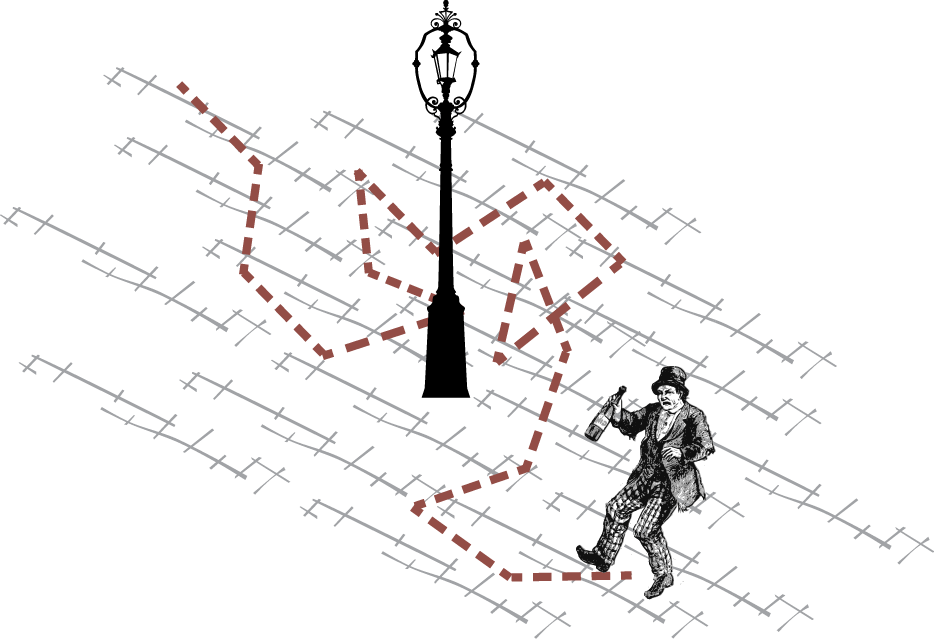
\includegraphics[width=0.8\linewidth]{../Figs/random_walk}
		%\caption{}
		\label{fig:random_walk}
	\end{figure}
\end{frame}

\begin{frame}\frametitle{Průběh jedné simulace}
	\begin{figure}
		\centering
		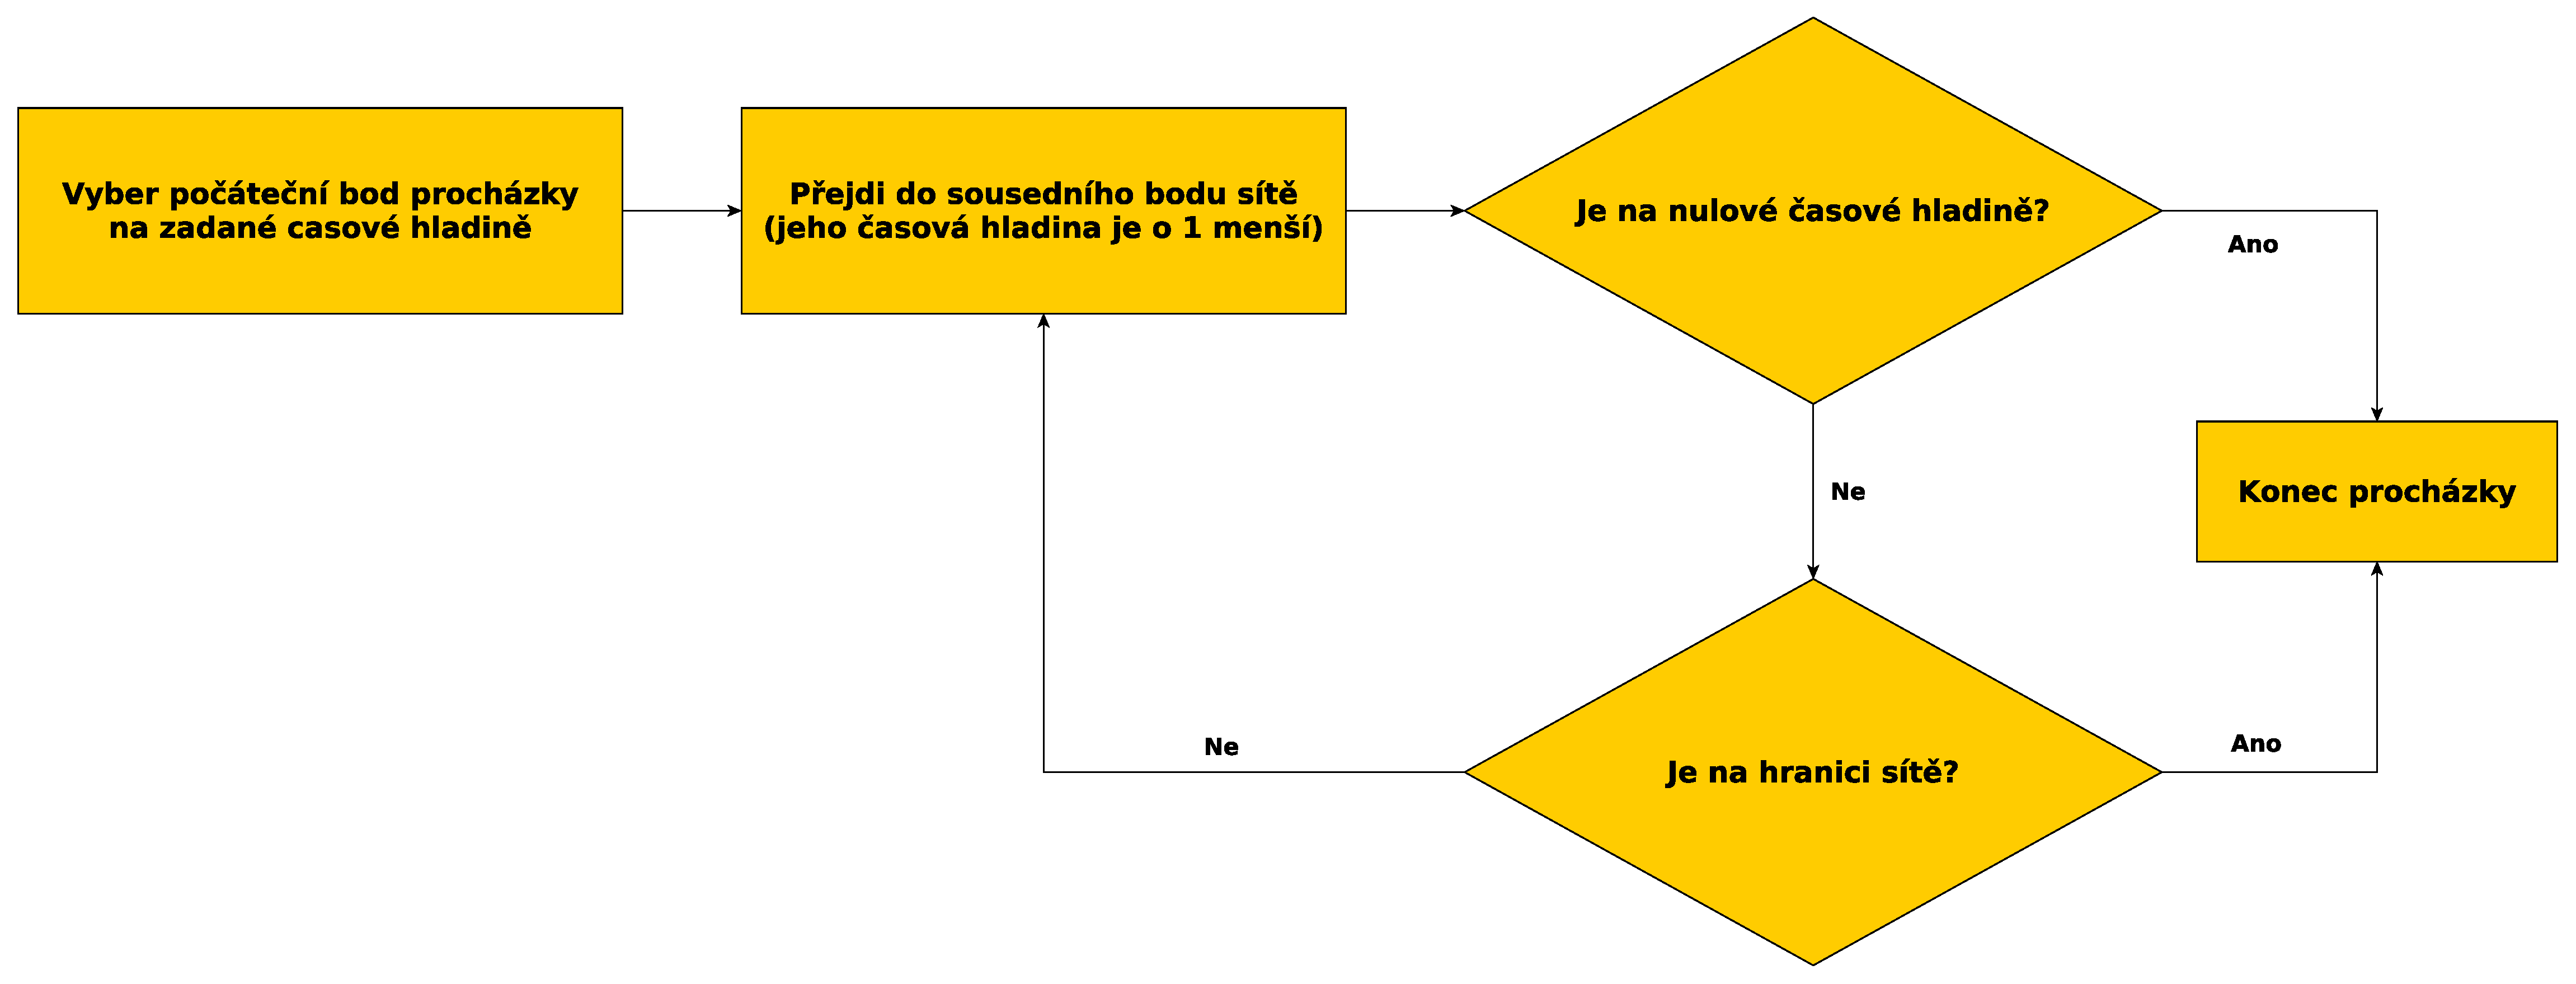
\includegraphics[width=1\linewidth]{../Figs/algorithm}
%		\caption{Průběh  jedné náhodné procházky}
		\label{fig:algorithm}
	\end{figure}

	$W_{ini}$ - počáteční bod náhodné procházky, $W_{fin}$ - její konečný bod, pak definujeme náhodnou veličinu $Y_{W_{ini}}$ následovně:
	\begin{itemize}
		\item $Y_{W_{ini}}=h(W_{fin})$, pokud $W_{fin}\in\omega_{h}$, ale $W_{fin}\notin\midpoint{\omega}_{h}$;
		\item $Y_{W_{ini}}=g(W_{fin})$, pokud $W_{fin}\in\midpoint{\omega}_{h}\setminus\omega_{h}$.
	\end{itemize}
\end{frame}



\section{Výsledky}

\subsection{Aproximace řešení diferenčního schématu}

\begin{frame}\frametitle{Nastavení parametrů:}
\begin{block}{}
\begin{itemize}
	\item krok sítě: $h=0.1$;
	\item časové hladiny: $k_{0}\in\{50,250\}$;
	\item okrajová podmínka: $g\equiv 273$;
	\item počáteční podmínka: $u(0,x)=h(x)=10x\cdot\exp(-x^2-y^2)+273$.
\end{itemize}
\end{block}

\begin{figure}[ht!]
\centering
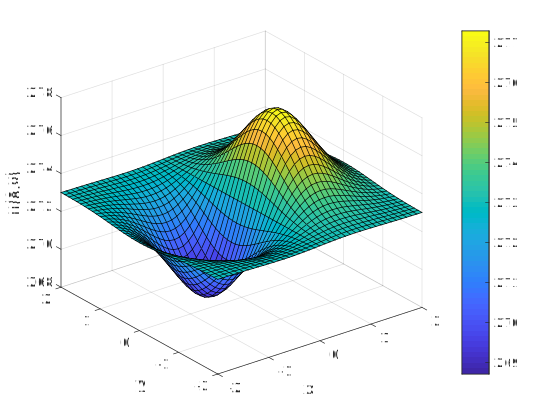
\includegraphics[width=0.55\linewidth]{../../results/initial_condition/initial_condition}
%\caption{Grafické znázornění počáteční podmínky \eqref{eq:initial_condition}.}
\label{fig:initial_condition}
\end{figure}

\end{frame}

\begin{frame}\frametitle{Počet simulací $N=100$}
\framesubtitle{časové hladiny $k_{0}=50$ (vlevo) a $k_{0}=250$ (vpravo)}
\begin{figure}
    \centering
    \begin{subfigure}[t]{0.5\textwidth}
        \centering
        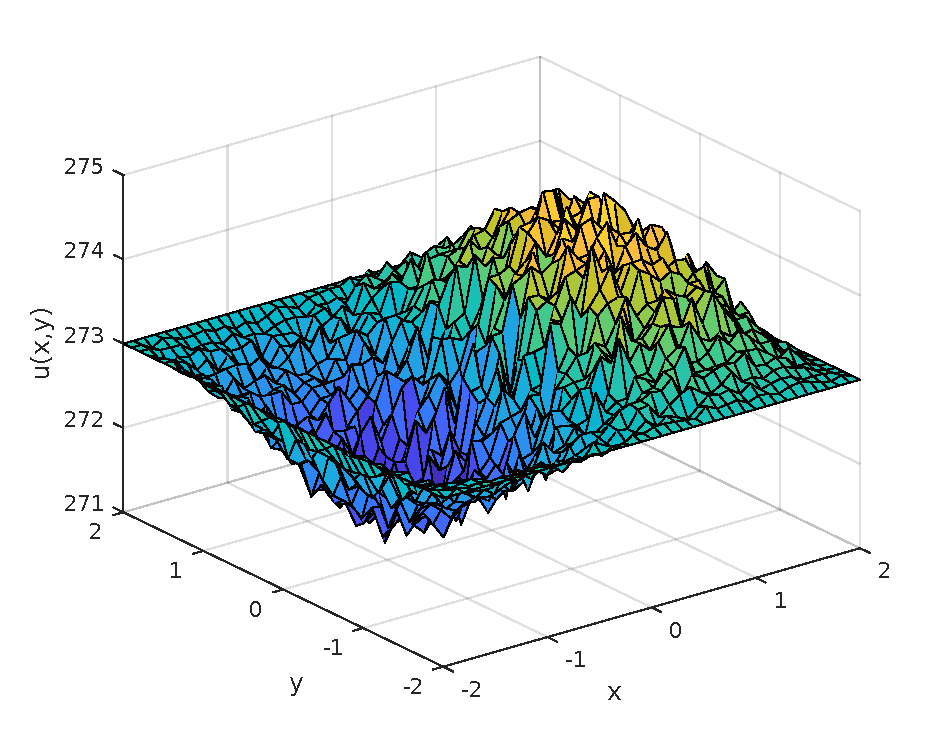
\includegraphics[width=0.75\linewidth]{../../results/simulations/100/solution_3D/solution_3D_sim100_step01_time50_boundary2.pdf}
%        \caption{Lorem ipsum}
    \end{subfigure}%
    ~ 
    \begin{subfigure}[t]{0.5\textwidth}
        \centering
        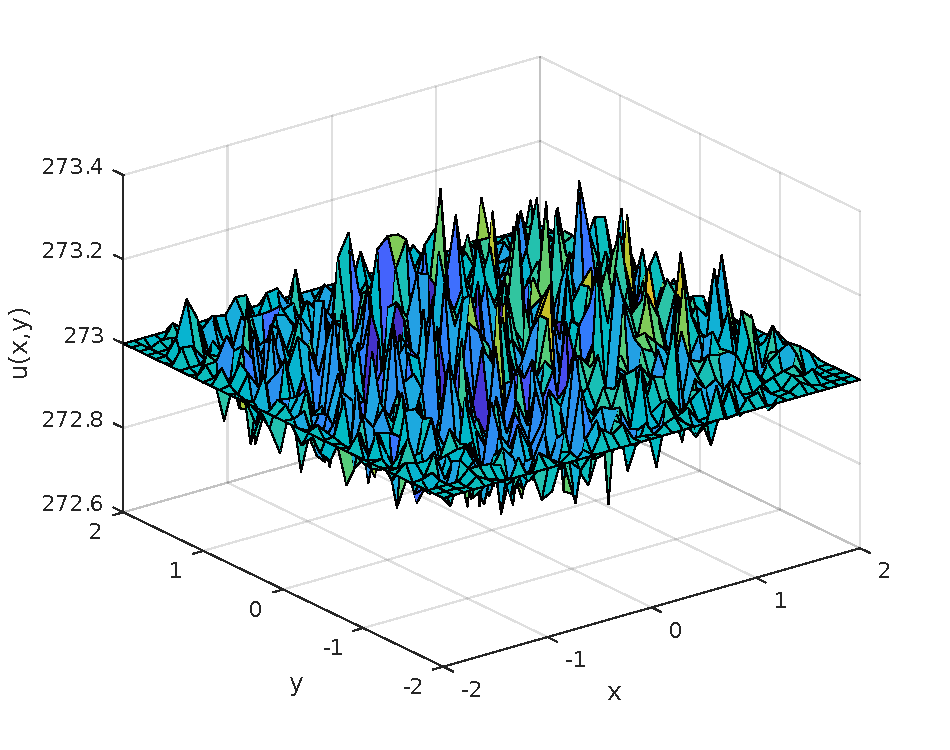
\includegraphics[width=0.75\linewidth]{../../results/simulations/100/solution_3D/solution_3D_sim100_step01_time250_boundary2.pdf}
%        \caption{Lorem}
    \end{subfigure}
    \begin{subfigure}[t]{0.5\textwidth}
        \centering
        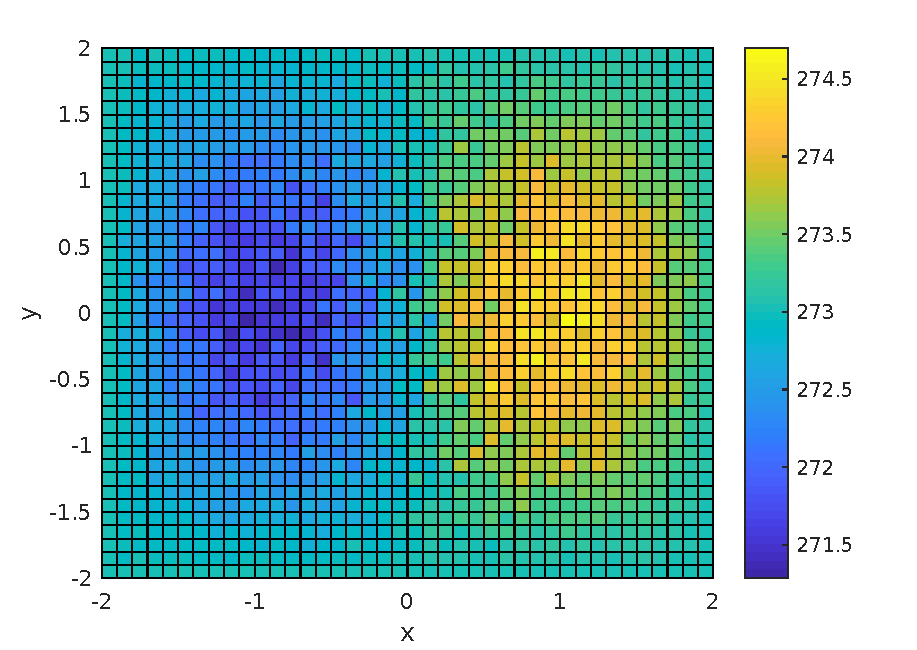
\includegraphics[width=0.775\linewidth]{../../results/simulations/100/solution_2D/solution_2D_sim100_step01_time50_boundary2.pdf}
%        \caption{Lorem ipsum}
    \end{subfigure}%
    ~ 
    \begin{subfigure}[t]{0.5\textwidth}
        \centering
        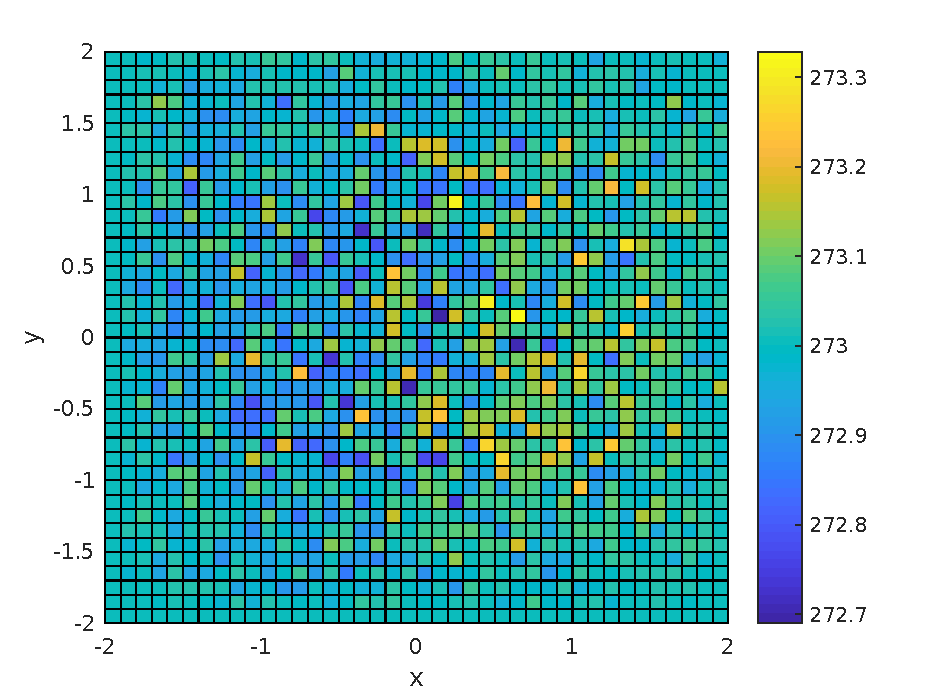
\includegraphics[width=0.725\linewidth]{../../results/simulations/100/solution_2D/solution_2D_sim100_step01_time250_boundary2.pdf}
%        \caption{Lorem}
    \end{subfigure}
%    \caption{Caption place holder}
\end{figure}
\end{frame}

\begin{frame}\frametitle{Počet simulací $N=1000$}
\framesubtitle{časové hladiny $k_{0}=50$ (vlevo) a $k_{0}=250$ (vpravo)}
\begin{figure}
    \centering
    \begin{subfigure}[t]{0.5\textwidth}
        \centering
        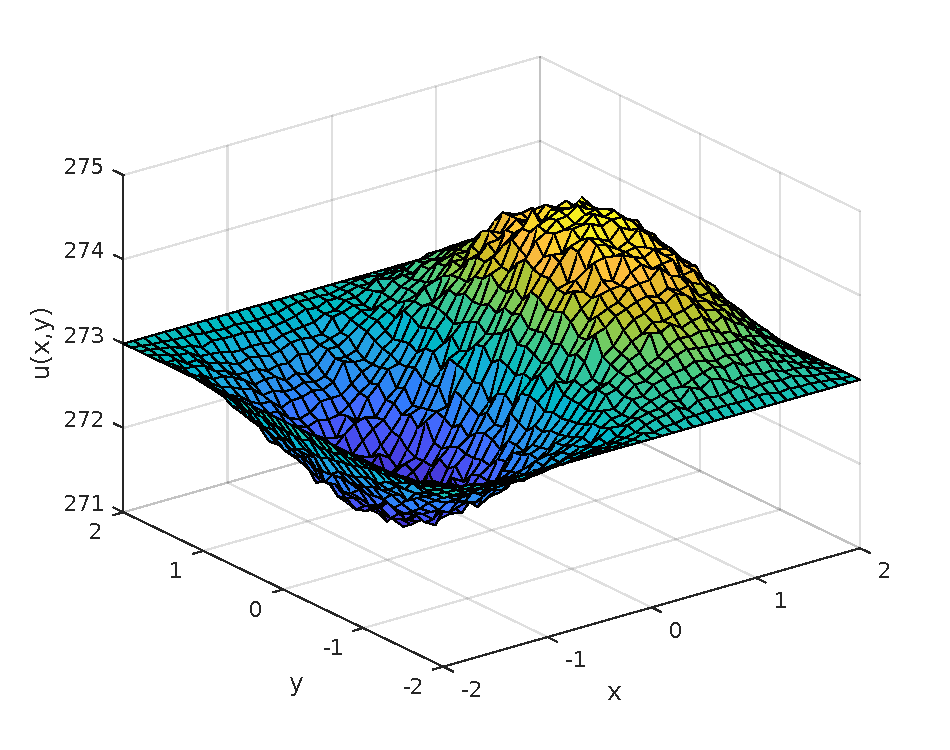
\includegraphics[width=0.75\linewidth]{../../results/simulations/1000/solution_3D/solution_3D_sim1000_step01_time50_boundary2.pdf}
%        \caption{Lorem ipsum}
    \end{subfigure}%
    ~ 
    \begin{subfigure}[t]{0.5\textwidth}
        \centering
        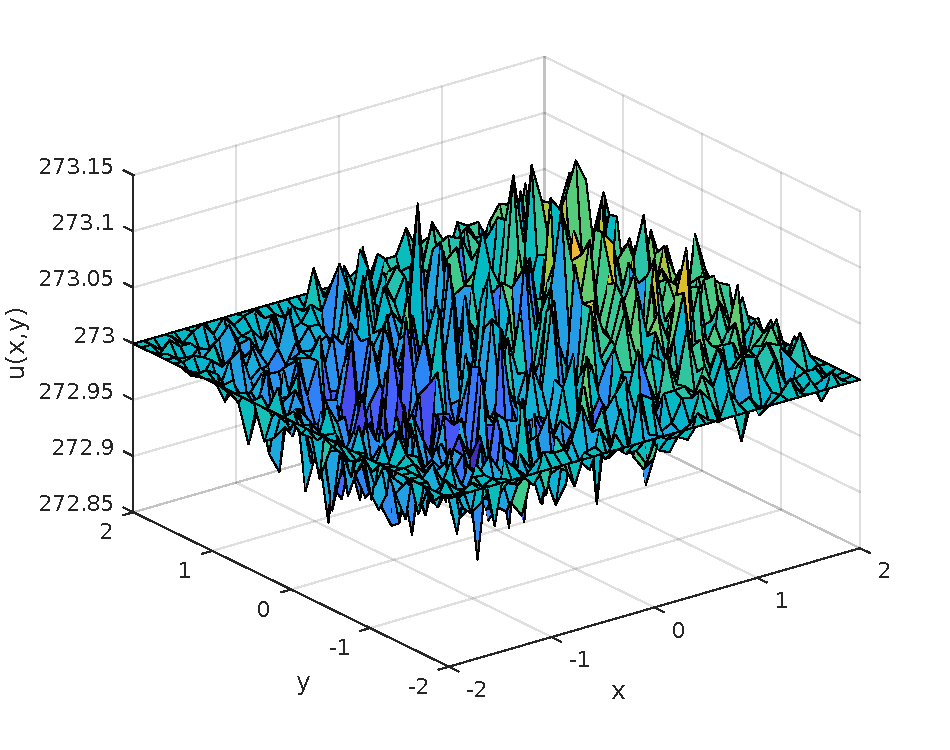
\includegraphics[width=0.75\linewidth]{../../results/simulations/1000/solution_3D/solution_3D_sim1000_step01_time250_boundary2.pdf}
%        \caption{Lorem}
    \end{subfigure}
    \begin{subfigure}[t]{0.5\textwidth}
        \centering
        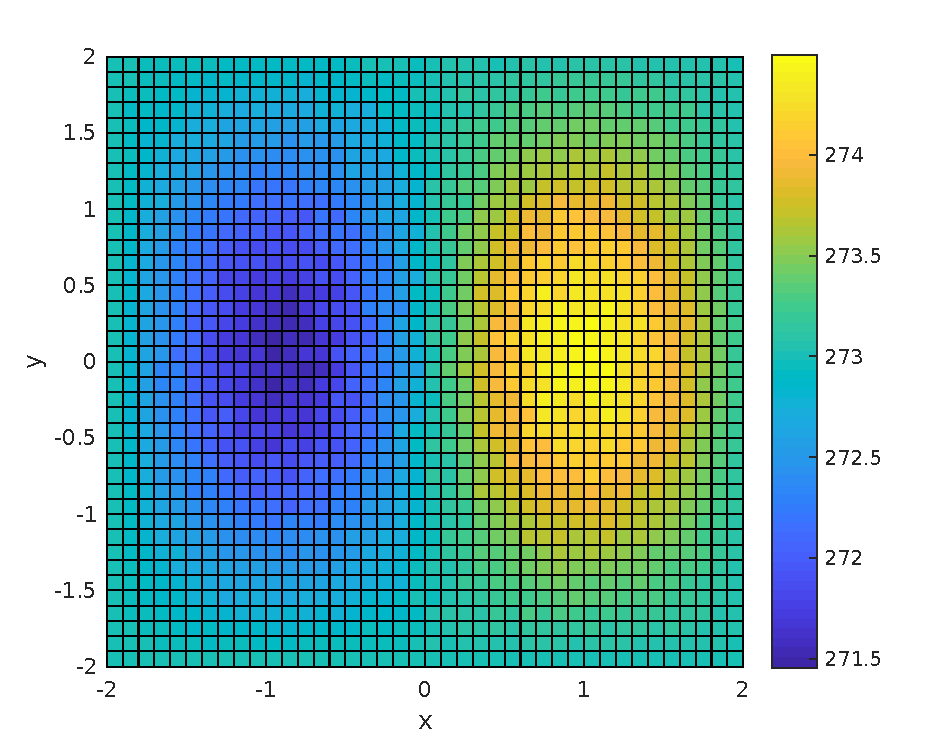
\includegraphics[width=0.70\linewidth]{../../results/simulations/1000/solution_2D/solution_2D_sim1000_step01_time50_boundary2.pdf}
%        \caption{Lorem ipsum}
    \end{subfigure}%
    ~ 
    \begin{subfigure}[t]{0.5\textwidth}
        \centering
        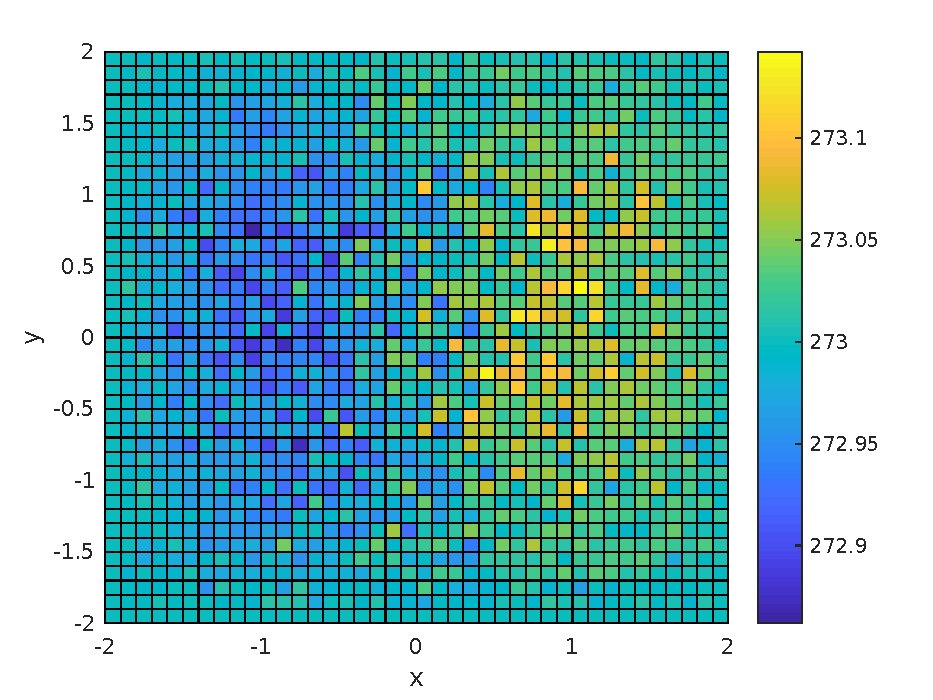
\includegraphics[width=0.725\linewidth]{../../results/simulations/1000/solution_2D/solution_2D_sim1000_step01_time250_boundary2.pdf}
%        \caption{Lorem}
    \end{subfigure}
%    \caption{Caption place holder}
\end{figure}
\end{frame}

\begin{frame}\frametitle{Počet simulací $N=10000$}
\framesubtitle{časové hladiny $k_{0}=50$ (vlevo) a $k_{0}=250$ (vpravo)}
\begin{figure}
    \centering
    \begin{subfigure}[t]{0.5\textwidth}
        \centering
        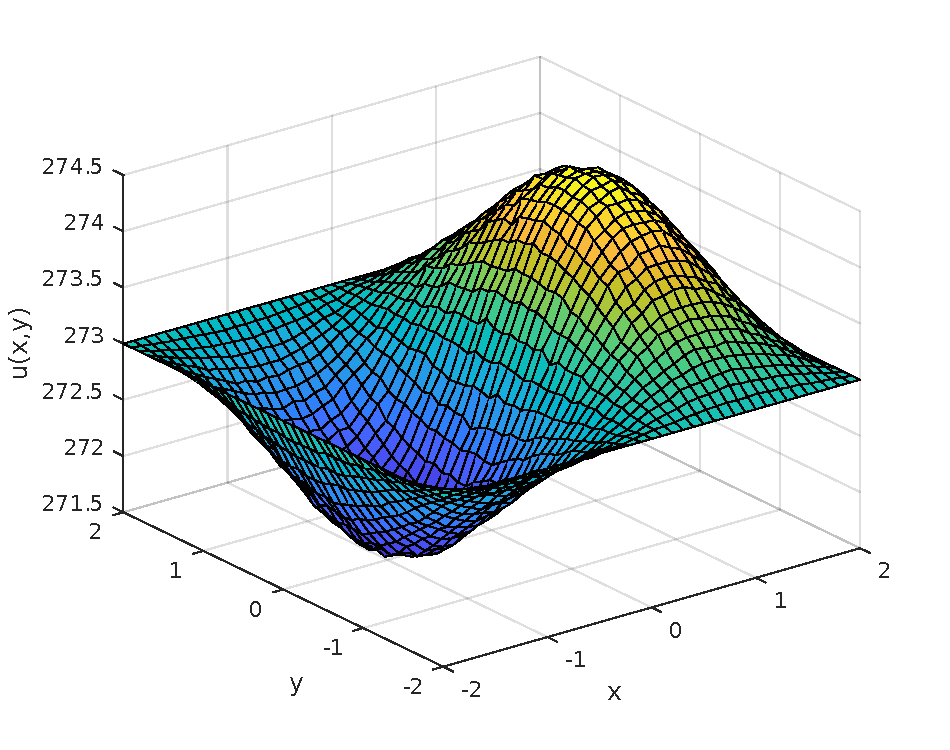
\includegraphics[width=0.75\linewidth]{../../results/simulations/10000/solution_3D/solution_3D_sim10000_step01_time50_boundary2.pdf}
%        \caption{Lorem ipsum}
    \end{subfigure}%
    ~ 
    \begin{subfigure}[t]{0.5\textwidth}
        \centering
        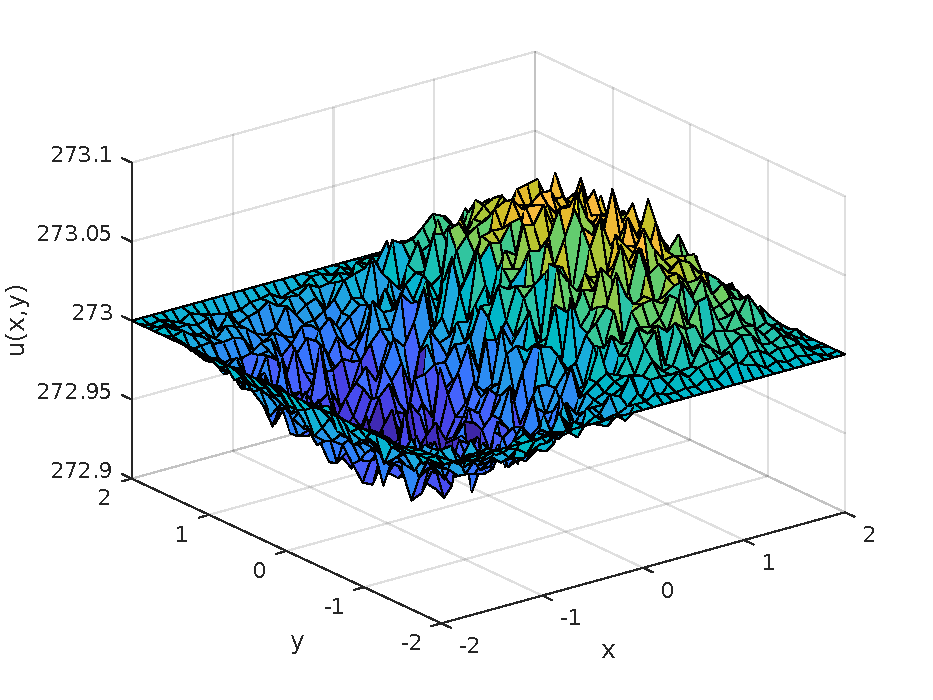
\includegraphics[width=0.75\linewidth]{../../results/simulations/10000/solution_3D/solution_3D_sim10000_step01_time250_boundary2.pdf}
%        \caption{Lorem}
    \end{subfigure}
    \begin{subfigure}[t]{0.5\textwidth}
        \centering
        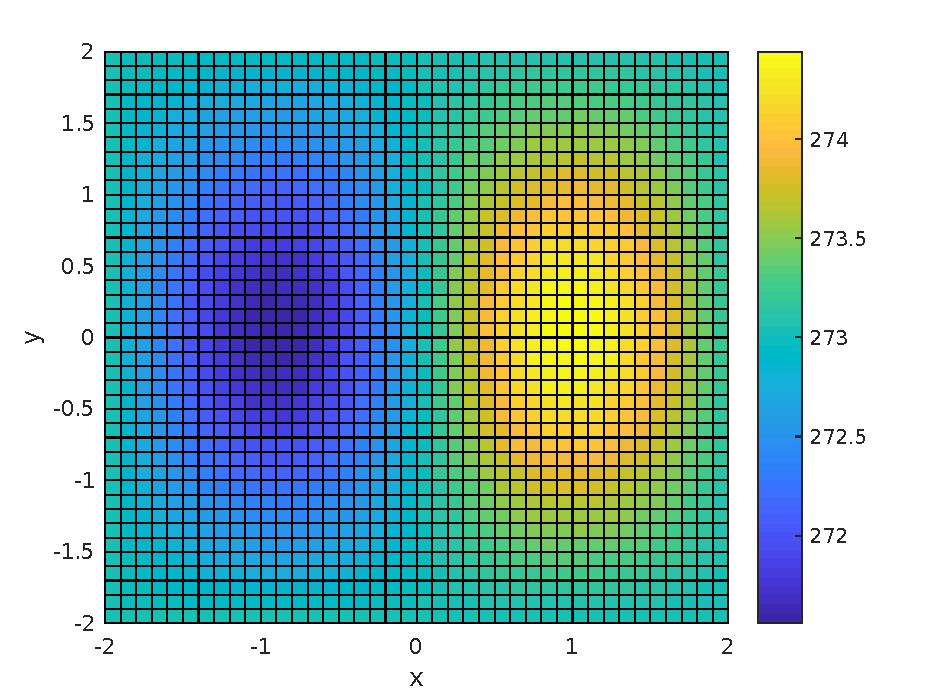
\includegraphics[width=0.725\linewidth]{../../results/simulations/10000/solution_2D/solution_2D_sim10000_step01_time50_boundary2.pdf}
%        \caption{Lorem ipsum}
    \end{subfigure}%
    ~ 
    \begin{subfigure}[t]{0.5\textwidth}
        \centering
        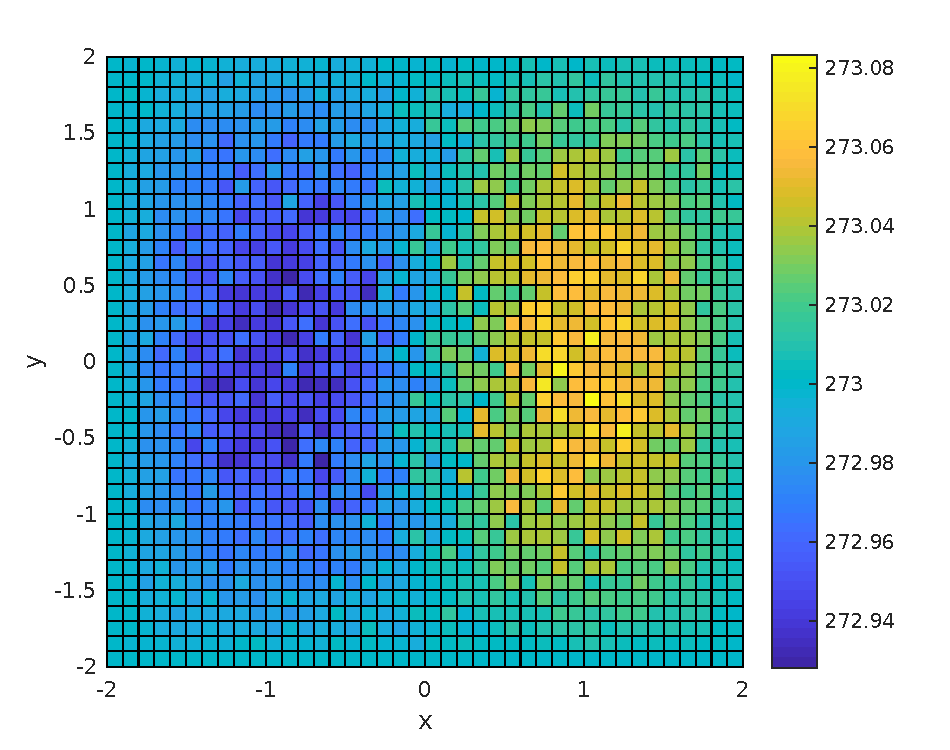
\includegraphics[width=0.71\linewidth]{../../results/simulations/10000/solution_2D/solution_2D_sim10000_step01_time250_boundary2.pdf}
%        \caption{Lorem}
    \end{subfigure}
%    \caption{Caption place holder}
\end{figure}
\end{frame}

\begin{frame}\frametitle{Počet simulací $N=100000$}
\framesubtitle{časové hladiny $k_{0}=50$ (vlevo) a $k_{0}=250$ (vpravo)}
\begin{figure}
    \centering
    \begin{subfigure}[t]{0.5\textwidth}
        \centering
        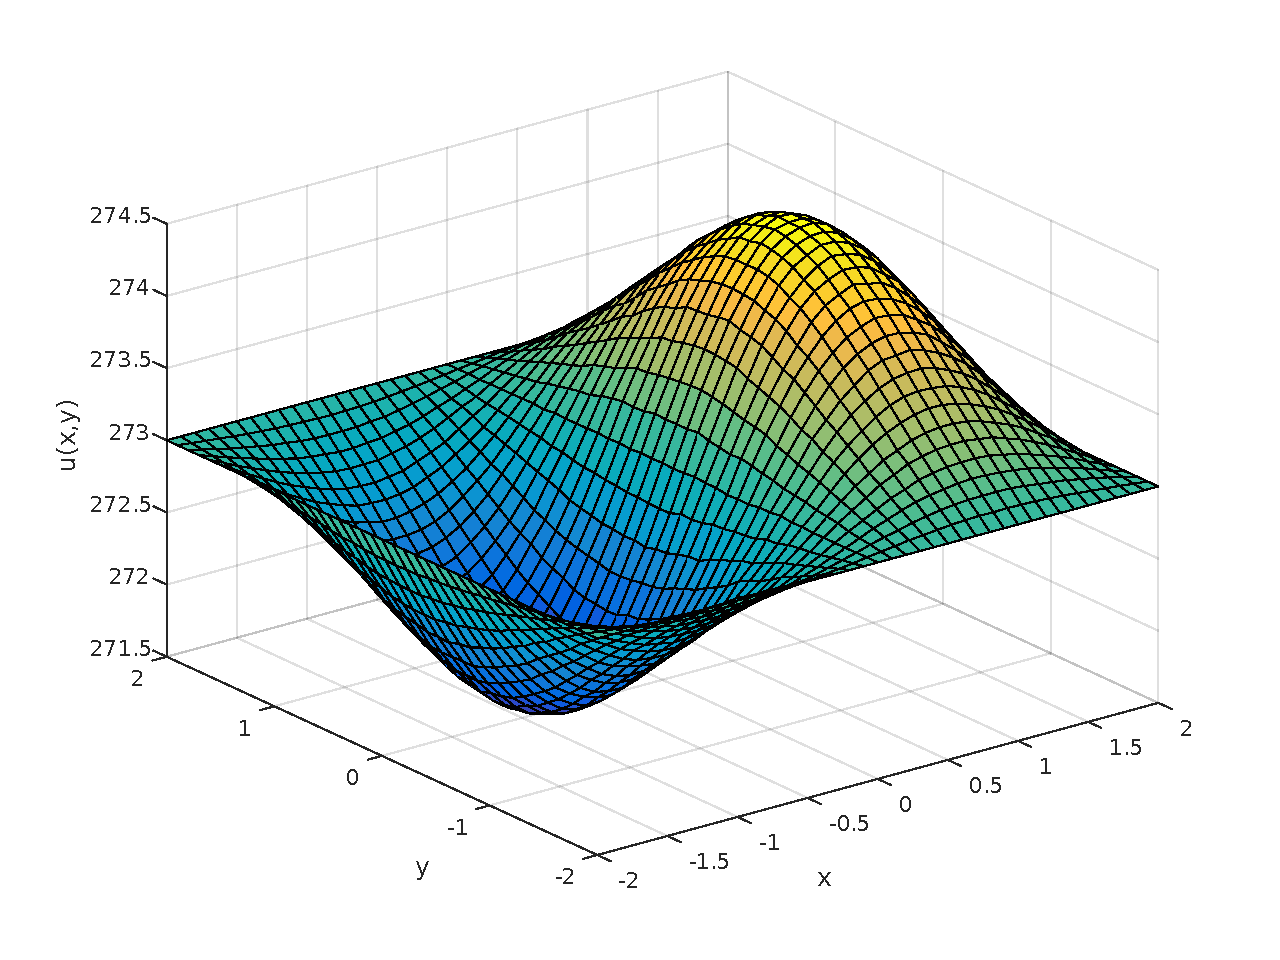
\includegraphics[width=0.775\linewidth]{../../results/simulations/100000/solution_3D/solution_3D_sim100000_step01_time50_boundary2.pdf}
%        \caption{Lorem ipsum}
    \end{subfigure}%
    ~ 
    \begin{subfigure}[t]{0.5\textwidth}
        \centering
        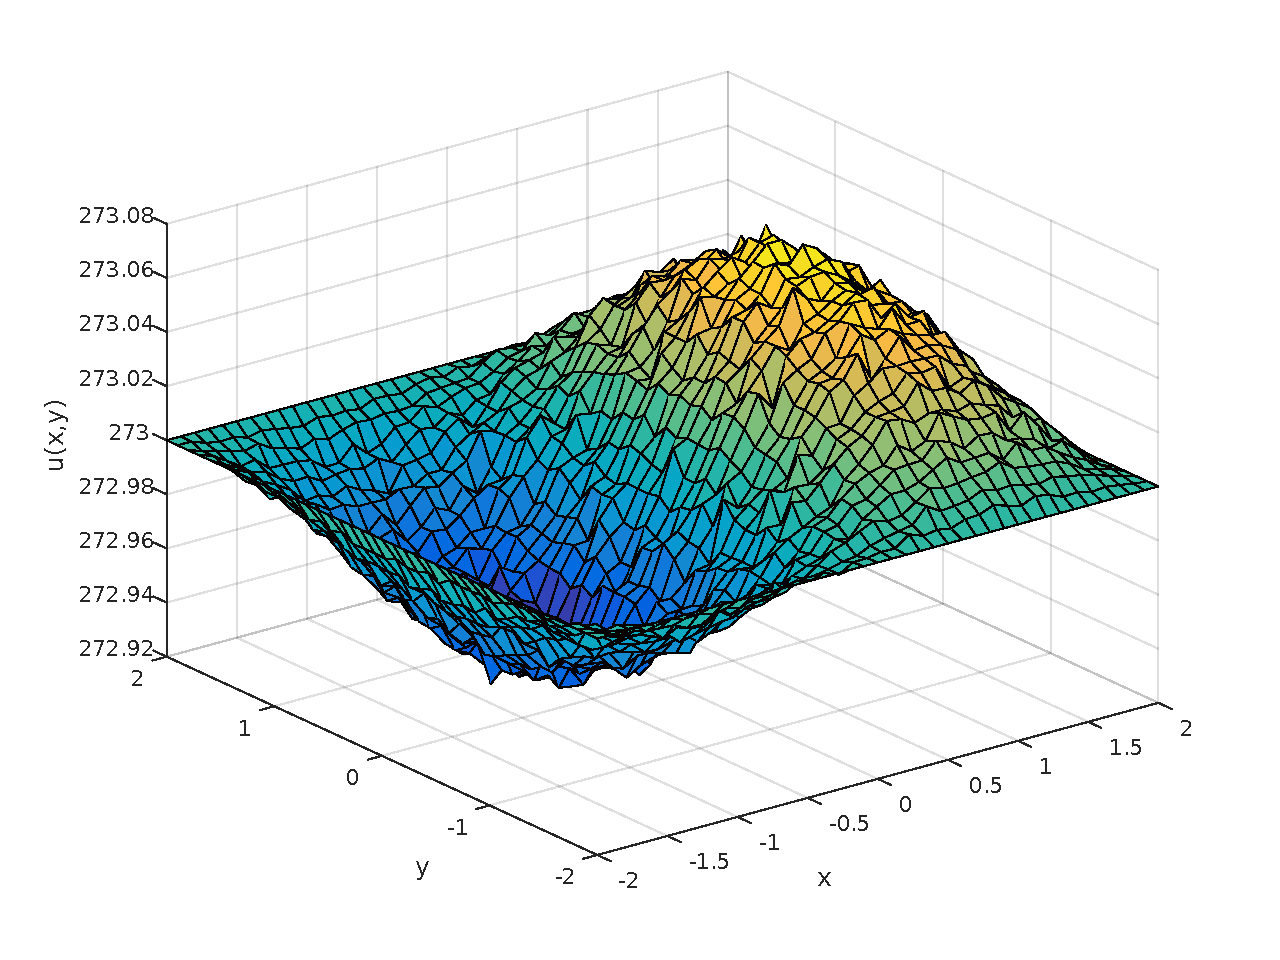
\includegraphics[width=0.775\linewidth]{../../results/simulations/100000/solution_3D/solution_3D_sim100000_step01_time250_boundary2.pdf}
%        \caption{Lorem}
    \end{subfigure}
    \begin{subfigure}[t]{0.5\textwidth}
        \centering
        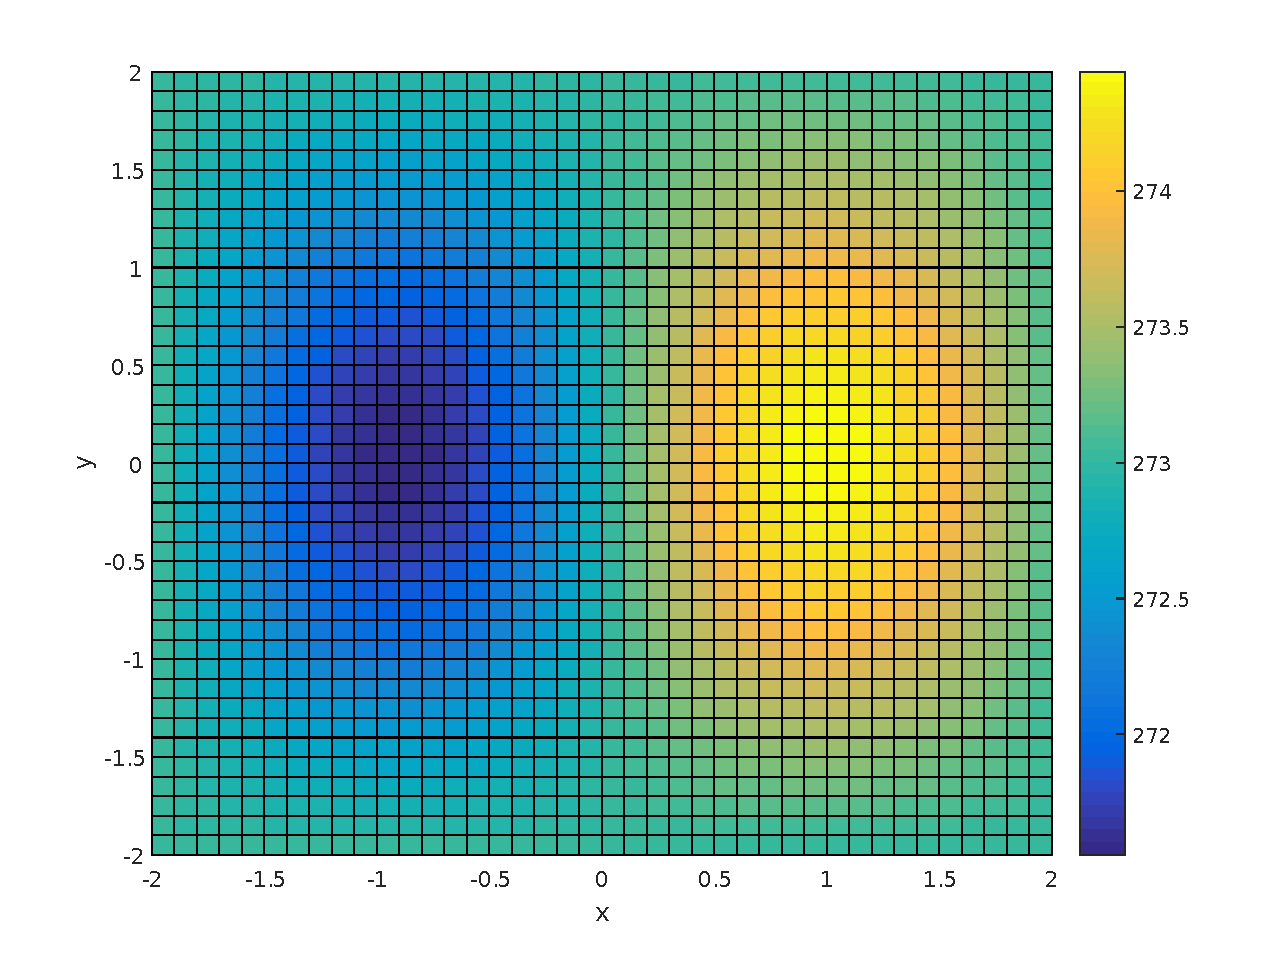
\includegraphics[width=0.75\linewidth]{../../results/simulations/100000/solution_2D/solution_2D_sim100000_step01_time50_boundary2.pdf}
%        \caption{Lorem ipsum}
    \end{subfigure}%
    ~ 
    \begin{subfigure}[t]{0.5\textwidth}
        \centering
        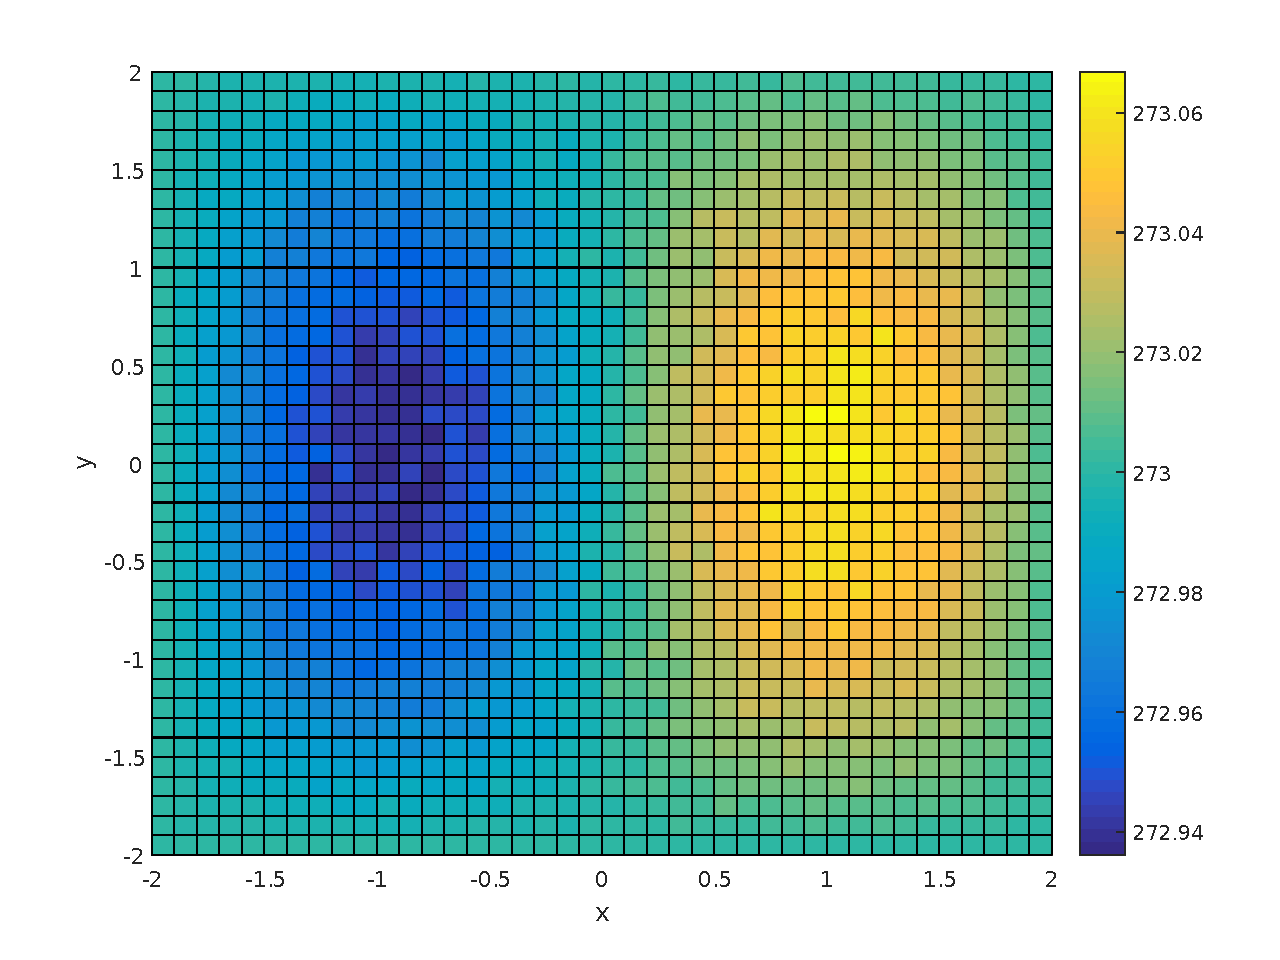
\includegraphics[width=0.75\linewidth]{../../results/simulations/100000/solution_2D/solution_2D_sim100000_step01_time250_boundary2.pdf}
%        \caption{Lorem}
    \end{subfigure}
%    \caption{Caption place holder}
\end{figure}
\end{frame}

\subsection{Chyba aproximace}

\begin{frame}\frametitle{Počet simulací $N=100$}
\framesubtitle{časové hladiny $k_{0}=50$ (vlevo) a $k_{0}=250$ (vpravo); hladina významnosti - $5 \%$}
\begin{figure}
    \centering
    \begin{subfigure}[t]{0.5\textwidth}
        \centering
        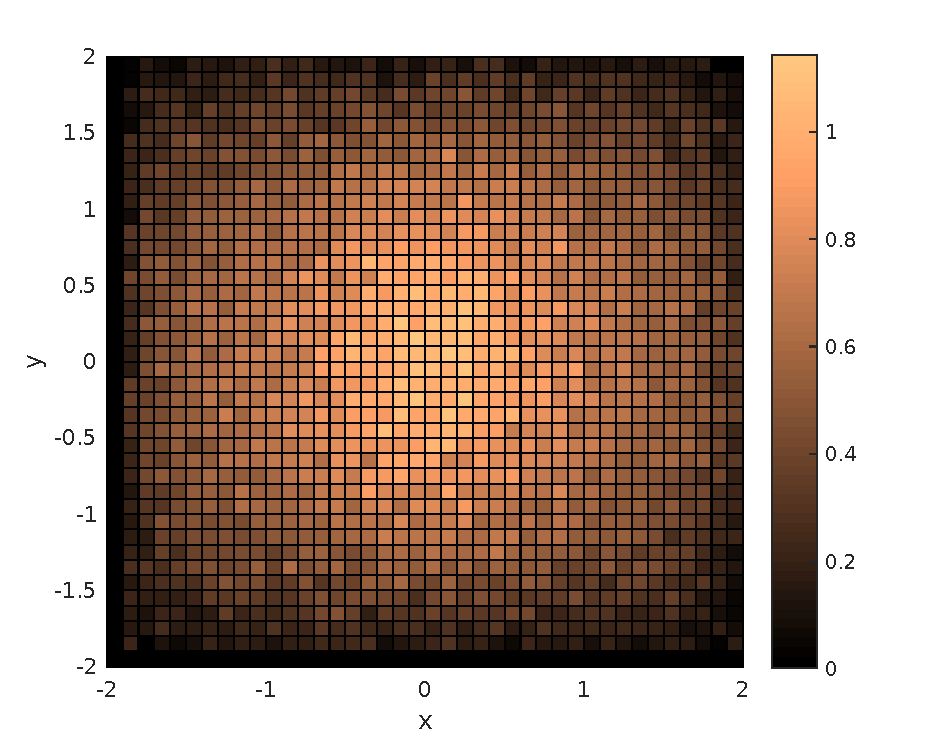
\includegraphics[width=1\linewidth]{../../results/simulations/100/solutionErr/solutionError_sim100_step01_time50_boundary2.pdf}
%        \caption{Lorem ipsum}
    \end{subfigure}%
    ~ 
    \begin{subfigure}[t]{0.5\textwidth}
        \centering
        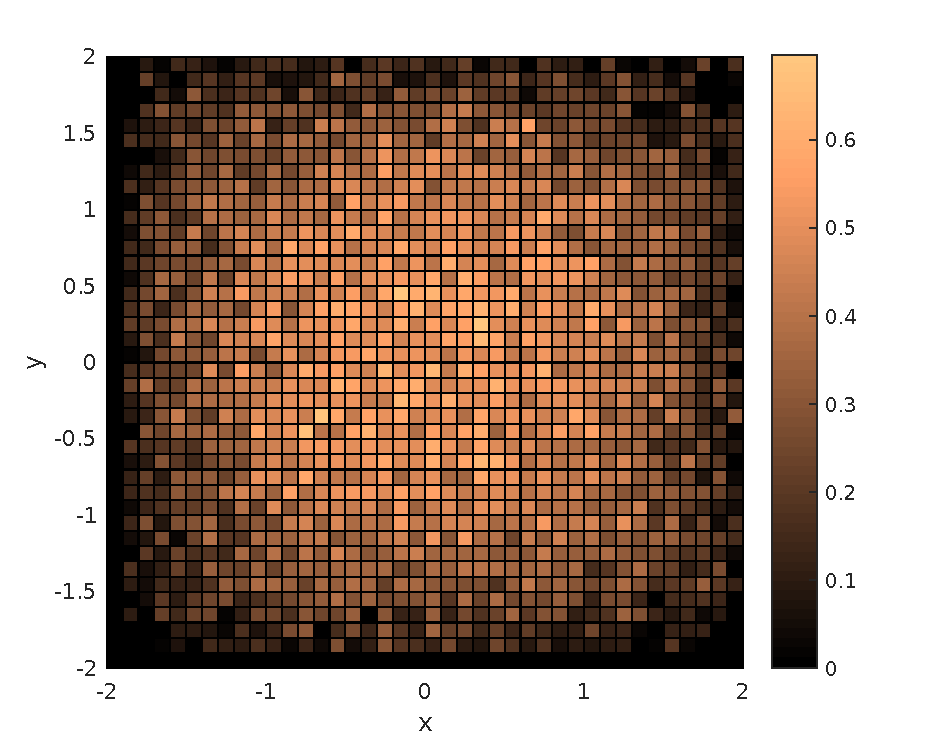
\includegraphics[width=1\linewidth]{../../results/simulations/100/solutionErr/solutionError_sim100_step01_time250_boundary2.pdf}
%        \caption{Lorem}
    \end{subfigure}
\end{figure}
\end{frame}

\begin{frame}\frametitle{Počet simulací $N=1000$}
\framesubtitle{časové hladiny $k_{0}=50$ (vlevo) a $k_{0}=250$ (vpravo); hladina významnosti - $5 \%$}
\begin{figure}
    \centering
    \begin{subfigure}[t]{0.5\textwidth}
        \centering
        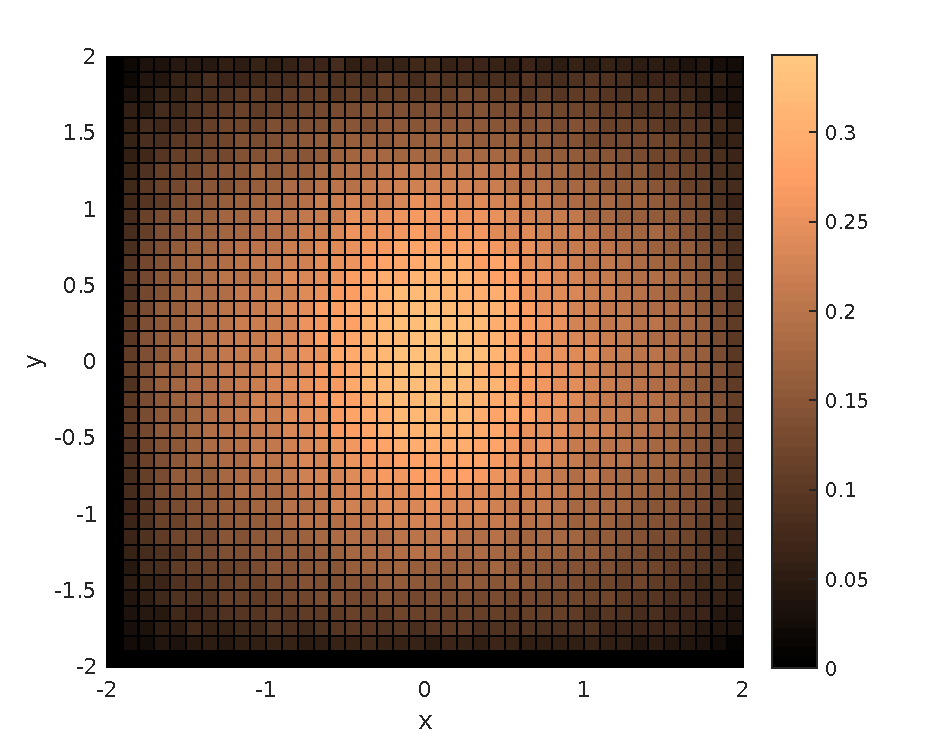
\includegraphics[width=1\linewidth]{../../results/simulations/1000/solutionErr/solutionError_sim1000_step01_time50_boundary2.pdf}
%        \caption{Lorem ipsum}
    \end{subfigure}%
    ~ 
    \begin{subfigure}[t]{0.5\textwidth}
        \centering
        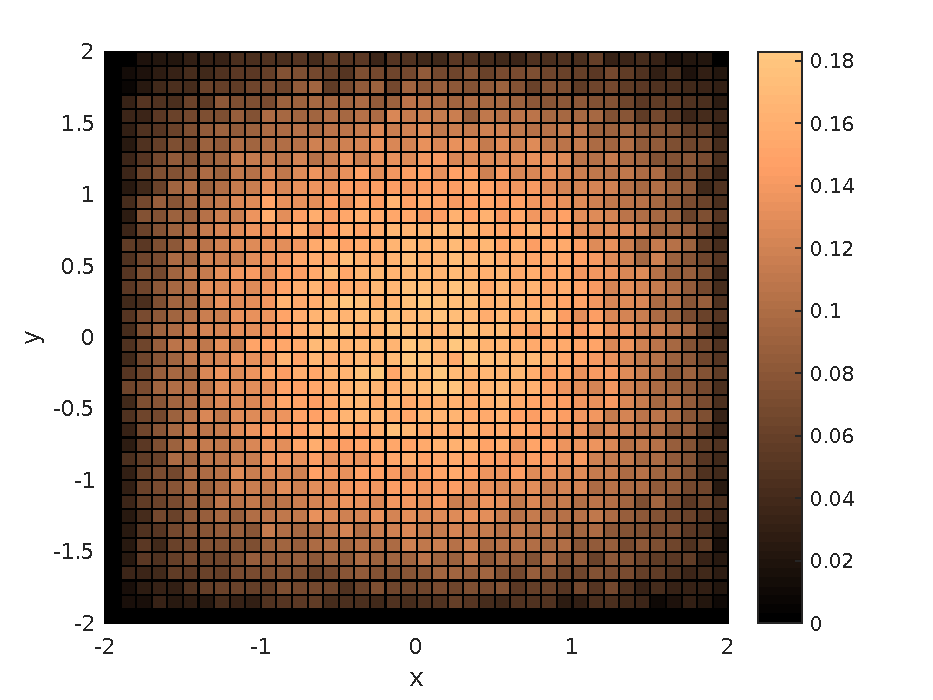
\includegraphics[width=1.05\linewidth]{../../results/simulations/1000/solutionErr/solutionError_sim1000_step01_time250_boundary2.pdf}
%        \caption{Lorem}
    \end{subfigure}
\end{figure}
\end{frame}

\begin{frame}\frametitle{Počet simulací $N=10000$}
\framesubtitle{časové hladiny $k_{0}=50$ (vlevo) a $k_{0}=250$ (vpravo); hladina významnosti - $5 \%$}
\begin{figure}
    \centering
    \begin{subfigure}[t]{0.5\textwidth}
        \centering
        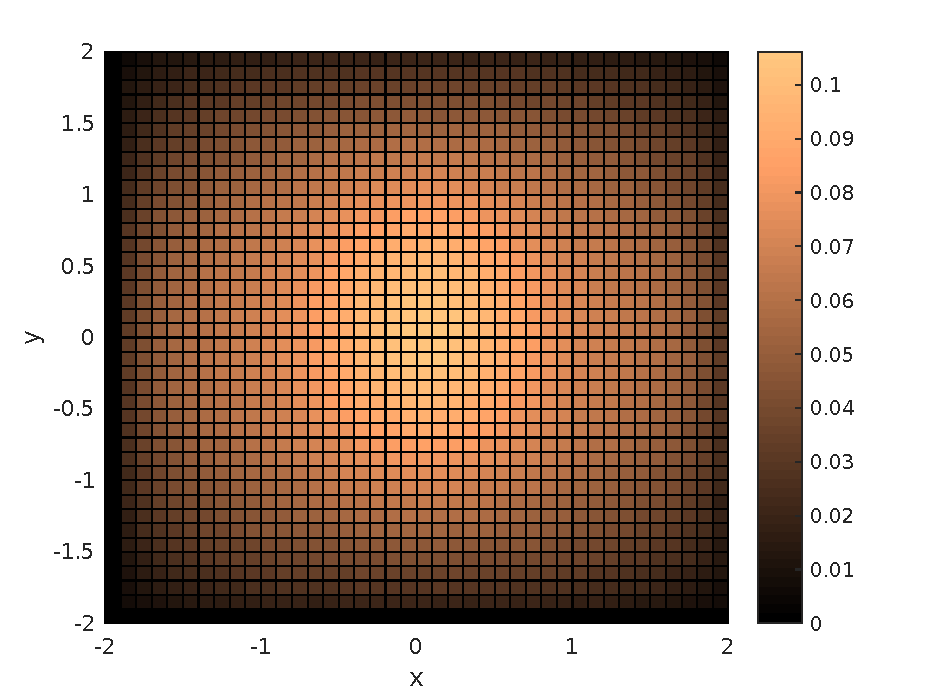
\includegraphics[width=1.05\linewidth]{../../results/simulations/10000/solutionErr/solutionError_sim10000_step01_time50_boundary2.pdf}
%        \caption{Lorem ipsum}
    \end{subfigure}%
    ~ 
    \begin{subfigure}[t]{0.5\textwidth}
        \centering
        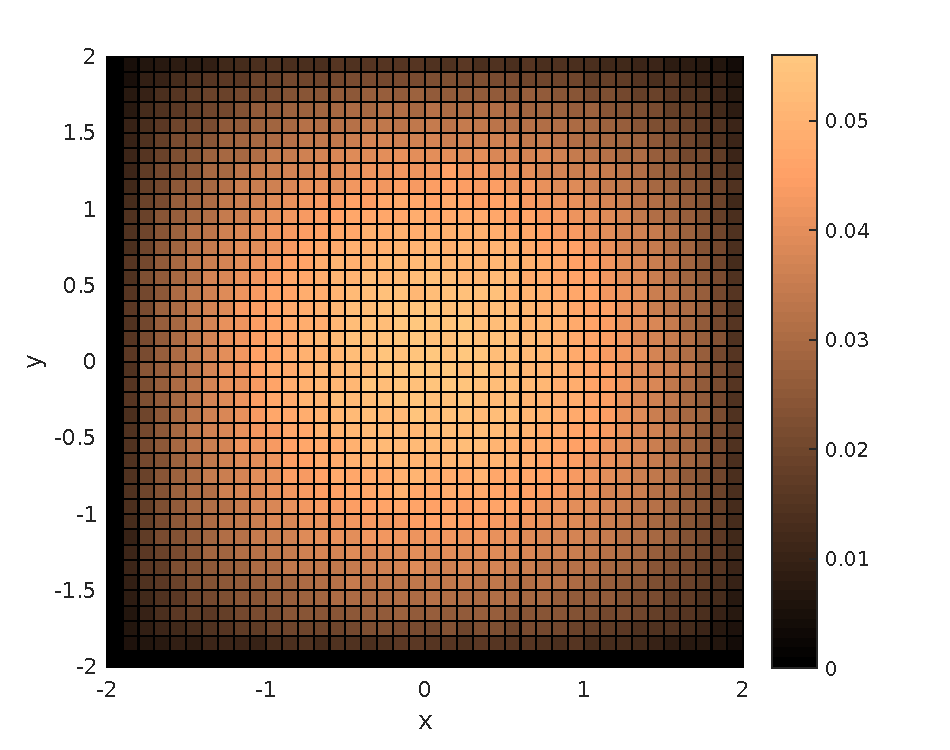
\includegraphics[width=1\linewidth]{../../results/simulations/10000/solutionErr/solutionError_sim10000_step01_time250_boundary2.pdf}
%        \caption{Lorem}
    \end{subfigure}
\end{figure}
\end{frame}

\begin{frame}\frametitle{Počet simulací $N=100000$}
\framesubtitle{časové hladiny $k_{0}=50$ (vlevo) a $k_{0}=250$ (vpravo); hladina významnosti - $5 \%$}
\begin{figure}
    \centering
    \begin{subfigure}[t]{0.5\textwidth}
        \centering
        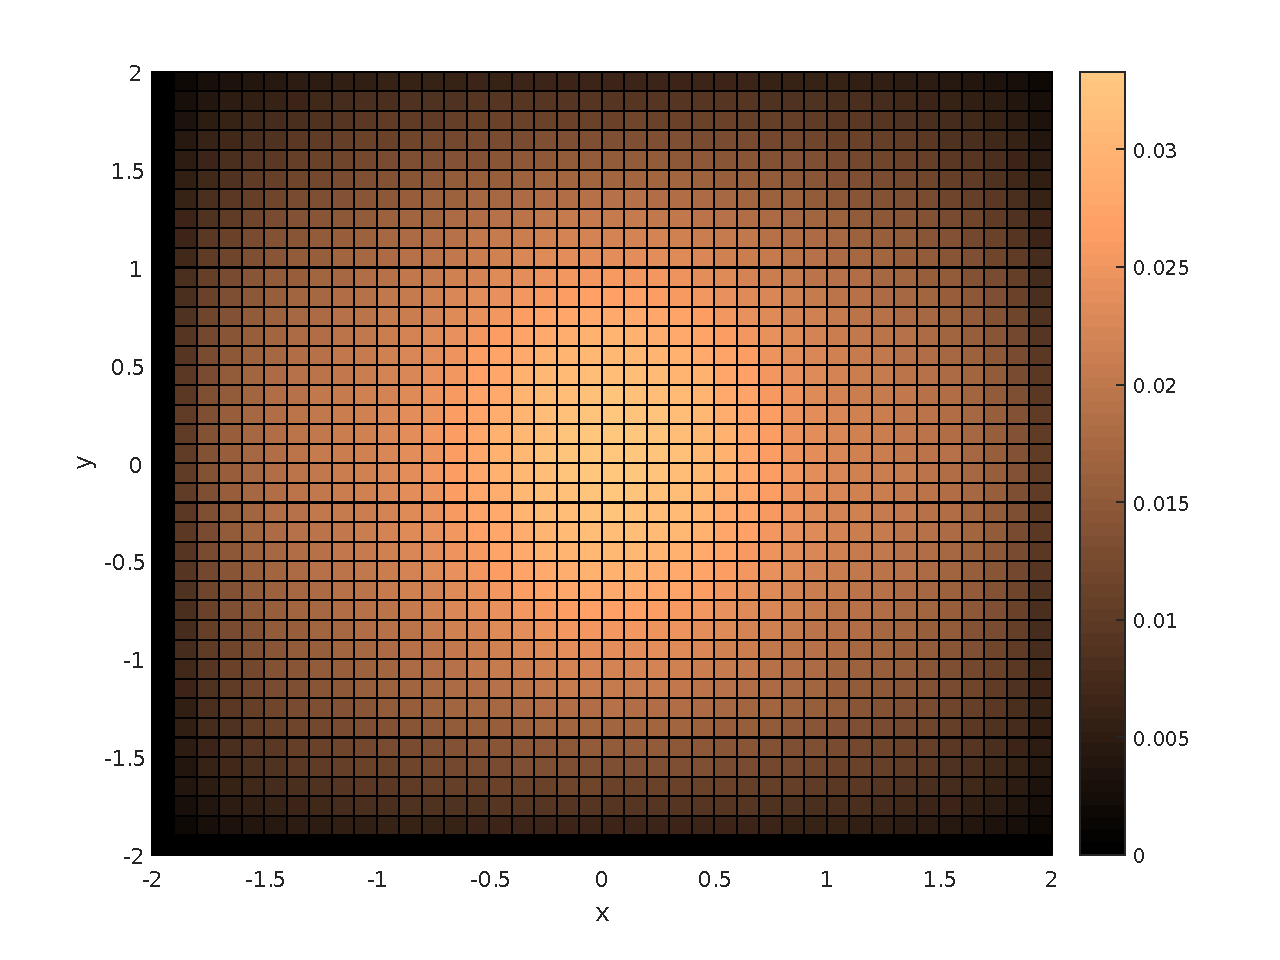
\includegraphics[width=1\linewidth]{../../results/simulations/100000/solutionErr/solutionError_sim100000_step01_time50_boundary2.pdf}
%        \caption{Lorem ipsum}
    \end{subfigure}%
    ~ 
    \begin{subfigure}[t]{0.5\textwidth}
        \centering
        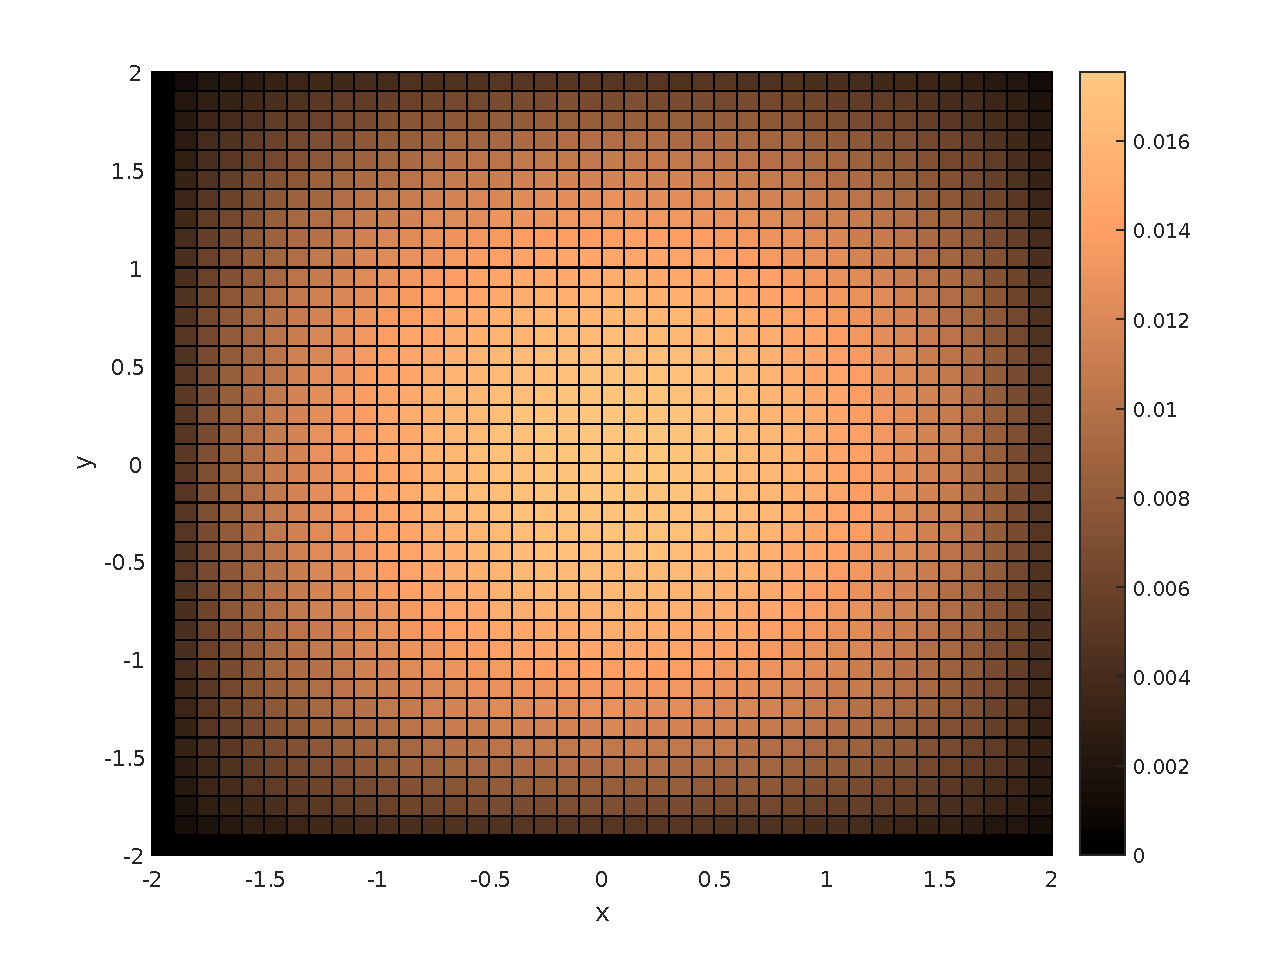
\includegraphics[width=1\linewidth]{../../results/simulations/100000/solutionErr/solutionError_sim100000_step01_time250_boundary2.pdf}
%        \caption{Lorem}
    \end{subfigure}
\end{figure}
\end{frame}

\begin{frame}\frametitle{Maximální chyba aproximace}
\framesubtitle{na hladině významnosti $5 \%$}

\begin{table}[H]
\renewcommand*{\arraystretch}{1.5}
\centering
	\begin{tabular}{ |c||c|c| }
		\hline
		Počet simulací, $N$ & Max. chyba, $k_{0}=50$ & Max. chyba, $k_{0}=250$ \\ \hline\hline
		$10^{\,2}$ & 1.1434 & 0.6963 \\ \hline
		$10^{\,3}$ & 0.3433 & 0.1830 \\ \hline
		$10^{\,4}$ & 0.1061 & 0.0560 \\ \hline
		$10^{\,5}$ & 0.0333 & 0.0176 \\ \hline
	\end{tabular}
	\caption{Maximální chyba aproximace řešení diskretizované parabolické evoluční úlohy pro časové hladiny $k_{0}\in\{50,250\}$.}
	\label{tab:error}
\end{table}
\end{frame}

\section{}

\begin{frame}
	\centering
	\Huge Děkuji za pozornost.
\end{frame}

%\nocite{*}
%
%\begin{frame}[allowframebreaks]\frametitle{Literatura}
%	{\scriptsize
%		\bibliography{../../Paper/BibTeX/Hart2001,../../Paper/BibTeX/Johnson2003,../../Paper/BibTeX/Challet1997,../../Paper/BibTeX/Moro2004,../../Paper/BibTeX/Minority_Games,../../Paper/BibTeX/Arthur1994,../../Paper/BibTeX/Johnson2014}
%		\bibliographystyle{alpha}
%	}
%\end{frame}


\end{document}